\documentclass[tikz,border=3pt]{standalone}
\usepackage{amssymb}
\usepackage{tikz}
\usetikzlibrary{arrows.meta,positioning}
\begin{document}
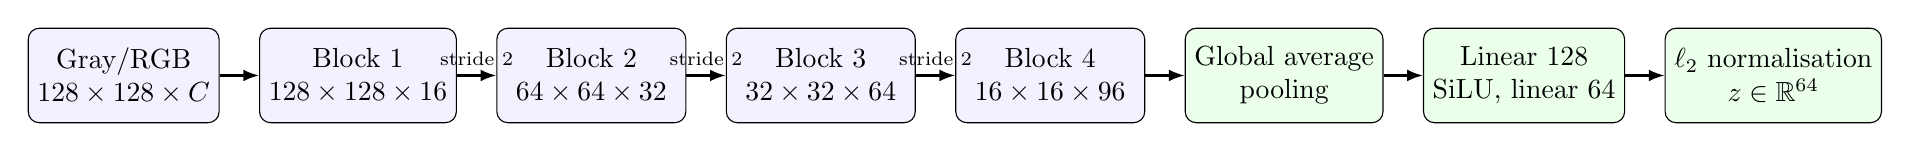
\begin{tikzpicture}[
  node distance=5mm,
  layer/.style={draw, rounded corners, align=center, minimum height=12mm,
    minimum width=24mm, fill=blue!5},
  head/.style={draw, rounded corners, align=center, minimum height=12mm,
    minimum width=21mm, fill=green!8},
  arrow/.style={-{Latex[length=2mm]}, thick}
]
\node[layer] (input) {Gray/RGB\\$128\times128\times C$};
\node[layer, right=of input] (b1) {Block 1\\$128\times128\times16$};
\node[layer, right=of b1] (b2) {Block 2\\$64\times64\times32$};
\node[layer, right=of b2] (b3) {Block 3\\$32\times32\times64$};
\node[layer, right=of b3] (b4) {Block 4\\$16\times16\times96$};
\node[head, right=of b4] (gap) {Global average\\pooling};
\node[head, right=of gap] (proj) {Linear 128\\SiLU, linear 64};
\node[head, right=of proj] (norm) {$\ell_2$ normalisation\\$z\in\mathbb{R}^{64}$};
\draw[arrow] (input)--(b1);
\draw[arrow] (b1)--node[above, font=\scriptsize]{stride 2}(b2);
\draw[arrow] (b2)--node[above, font=\scriptsize]{stride 2}(b3);
\draw[arrow] (b3)--node[above, font=\scriptsize]{stride 2}(b4);
\draw[arrow] (b4)--(gap);
\draw[arrow] (gap)--(proj);
\draw[arrow] (proj)--(norm);
\end{tikzpicture}
\end{document}
